%%
%%  Department of Electrical, Electronic and Computer Engineering.
%%  EPR400/2 Final Report - Section 1.
%%  Copyright (C) 2011-2021 University of Pretoria.
%%

\section{Literature study}

Malaria is still one of the leading causes of death in low-income countries according to the World Health Organisation \cite{WHO2020}. Mosquitoes that do not carry diseases are also a general nuisance in the everyday life of people living in mosquito-prone areas. The main defence mechanism employed against mosquitoes are mosquito repellents. Mosquito repellents do provide a certain degree of relief against pestering mosquitoes, however repellents only provide temporary relief. Electric insect killers is the other main defence mechanism employed against mosquitoes. These devices use ultraviolet light to attract insects and electrocute them when they come into contact with an electrified grid or a similar mechanism. The devices are obtrusive and ineffective on mosquitoes that were not attracted by the ultraviolet light. Therefore, it is necessary to pursue improvement in our defence against mosquitoes. A laser turret based mosquito defence system could prove to be an unobtrusive and effective defence mechanism against mosquitoes.

The successful development of such a mosquito defence system will require accurate detection and tracking of mosquitoes. The tracking of mosquitoes is a challenging task because of the small size of mosquitoes and their erratic flight patterns. The detection and tracking solutions investigated will be based on camera imaging. There are two main approaches to object tracking: appearance-based tracking and tracking-by-detection. Appearance based tracking approaches utilise the appearance of the object directly in the tracking process, while tracking-by-detection approaches rely on an external object detectors.

Deep learning object detection algorithms have been shown to be effective in detecting objects based on appearance. Creating a deep learning detection algorithm require large sets of training data. Collecting a large set of mosquito images for training will be a challenging task. A popular deep learning object detection and identification system is the YOLOv3 algorithm. Appearance based detection can also be applied using a pattern matching approach. In general pattern matching is searching and checking images for the presence of other given images (patterns) to find and mark the patterns' locations (if any) within the given images. Appearance based detection models require high quality image data since the detection is based on appearance. This can be highly beneficial when features can be extracted from an object's appearance or the object's orientation can be estimated based on its appearance. The study conducted by Hurtik et al. \cite{Hurtik2018} presents results based on F-transform pattern matching. The best operating frame rate that was achieved in \cite{Hurtik2018} was 0.43 frames per second. This is far too slow to be used in a real-time tracking applications. A frame rate of at least 5 frames per second is required to achieve good real-time performance especially when the tracking subject exhibits erratic behaviour such as a mosquito. Appearance based detection and tracking approaches are only viable for mosquitoes when imaged close-up. A laser turret mosquito targeting system is not feasible when close-up imaging is required to detect and track mosquitoes. This is because the laser turret will be required to target mosquitoes over a large area in order for it to be effective. Therefore, appearance based detection and tracking approaches will not be suitable for the proposed mosquito defence system.

An alternative to the appearance based detection approaches is to detect objects by isolating the background and foreground of the image \cite{Liang2016}. The laser turret based mosquito defence system will be developed to operate in a controlled environment. The background of the environment will exhibit little to no change and will be uniform. This will enable the background of the image to be isolated from the foreground. The foreground of the image should only contain the objects of interest. In \cite{Bao2018}, a dual foreground and background model is proposed to improve mosquito detection accuracy. This should not be required for laser turret mosquito defence system since the mosquitoes will be in a controlled environment. Detected objects that are too close to one another are split into two, and abnormally small objects are merged in \cite{Bao2018}.

Tracking-by-detection approaches are more suitable for the proposed mosquito defence system. Tracking-by-detection approaches are based on the detection of objects in a scene and the tracking of the detected objects. Tracking-by-detection can be performed using particle filter-based tracking. A particle filter considers the proximity and behaviour of other targets. In the case of social insect tracking, it is known that two targets cannot occupy the same space, and targets will actively avoid collisions. The joint particle tracker proposed in \cite{Khan2003} is highly accurate but unfortunately, it suffers from exponential complexity. This computational complexity is not feasible in real-time multi-target tracking system.

The \gls{sort} algorithm proposed in \cite{SORT-Bewley2017} has a main focus to associate objects efficiency for online and real-time applications. The \gls{sort} uses the combination of a Kalman filter and the Hungarian algorithm. The Kalman filter is an optimal linear state estimator. The Hungarian algorithm is an optimal assignment algorithm. The performance of the \gls{sort} algorithm can be seen in \autoref{fig:sort_performance}.
\begin{figure}[h]
  \centering
  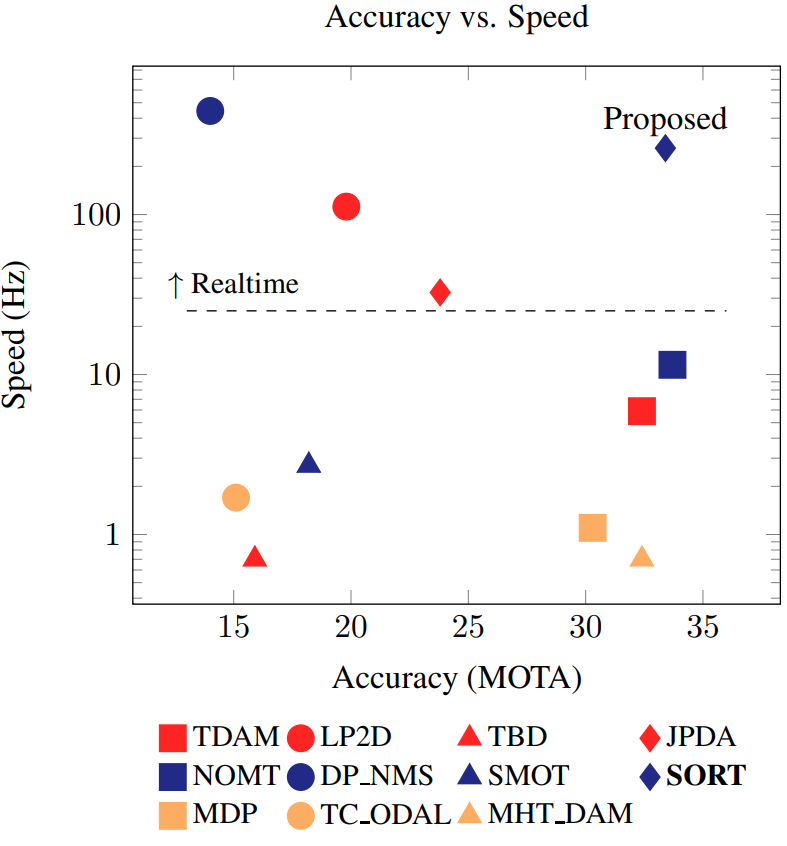
\includegraphics[width=0.6\textwidth]{figures/sort_performance.png}
  \caption{Performance of the \gls{sort} algorithm \cite{SORT-Bewley2017}.}
  \label{fig:sort_performance}
\end{figure}
The \gls{sort} algorithm employs a Kalman filter for each object that is being tracked. The Kalman filter is used to predict the future location of the object. The Hungarian algorithm is used to assign detections to tracks. The Kalman filter requires a series of matrix operations to be performed for each object that is being tracked. The Hungarian algorithm has a time complexity of $O\left(n!\right)$. The computational complexity of the \gls{sort} tracking makes it suitable for the proposed mosquito defence system.

The laser pointer turret based mosquito air defence system will be developed using a tracking-by-detection paradigm. The appearance based detection approaches are not suitable for the proposed system because of the small size of mosquitoes and the large area that the laser turret will be required to cover. The mosquito detection system will be design using a background and foreground isolation approach similar to the approaches described in \cite{Liang2016} and \cite{Bao2018}. The computational complexity of particle filter based tracking approaches make them infeasible for real-time requirements of the system. The tracking system will be based on the \gls{sort} algorithm proposed in \cite{SORT-Bewley2017}. The \gls{sort} algorithm is ideally suited for laser turret mosquito defence system since it was designed to be implemented in online real-time systems.

\newpage

%% End of File.


